\documentclass{thesisclass}

%% -------------------------------
%% |    ISSD Thesis Template       |
%% -------------------------------
%% Further additions by:
%%   Philipp Stroehle, IM, 2013 
%%   Jasper Feine, ISSD, 2018
%%   Merlin Knaeble, ISSD, 2020-2022 
%% firstname.lastname "at" kit.edu

%% Notes:
%% Language switch after \begin{document}

% Based on thesisclass.cls of Timo Rohrberg, 2009
% ----------------------------------------------------------------
% Thesis - Main document
% ----------------------------------------------------------------

\usepackage[english]{babel}
\usepackage{csquotes}

%% ---------------------------------
%% |      Additional packages      |
%% ---------------------------------
%% 

\usepackage{graphicx}
\DeclareGraphicsExtensions{.pdf,.png,.jpg}
\graphicspath{{./figures/}} %Use curly braces for each path to add and don't forget trailing slash '/'
% \usepackage{epstopdf} %Nice to automatically convert eps figures to pdf format  (from inkscape, etc)
\usepackage[style=apa, backend=biber, natbib=true, hyperref=true, uniquelist=true, language=american]{biblatex}
%\addbibresource{thesis.bib}
\usepackage{booktabs}

%% ---------------------------------
%% | Needed for the List of Abbreviations |
%% ---------------------------------
\usepackage{nomencl}
\renewcommand{\nomname}{List of Abbreviations}
\setlength{\nomlabelwidth}{.40\hsize}
\renewcommand{\nomlabel}[1]{#1 \dotfill}
\setlength{\nomitemsep}{-\parsep}
\makenomenclature
\usepackage[normalem]{ulem}
\newcommand{\markup}[1]{\uline{#1}}

\usepackage{listings}
\usepackage{xcolor}
\usepackage{svg}

\lstdefinelanguage{json}{
    basicstyle=\ttfamily,
    numbers=left,
    numberstyle=\tiny\color{gray},
    stepnumber=1,
    numbersep=8pt,
    showstringspaces=false,
    breaklines=true,
    frame=lines,
    backgroundcolor=\color{lightgray},
    literate=
     *{0}{{{\color{blue}0}}}{1}
      {1}{{{\color{blue}1}}}{1}
      {2}{{{\color{blue}2}}}{1}
      {3}{{{\color{blue}3}}}{1}
      {4}{{{\color{blue}4}}}{1}
      {5}{{{\color{blue}5}}}{1}
      {6}{{{\color{blue}6}}}{1}
      {7}{{{\color{blue}7}}}{1}
      {8}{{{\color{blue}8}}}{1}
      {9}{{{\color{blue}9}}}{1}
      {:}{{{\color{red}{:}}}}{1}
      {,}{{{\color{red}{,}}}}{1}
      {\{}{{{\color{orange}{\{}}}}{1}
      {\}}{{{\color{orange}{\}}}}}{1}
      {[}{{{\color{orange}{[}}}}{1}
      {]}{{{\color{orange}{]}}}}{1},
}
\usepackage{amsmath}

\lstdefinestyle{bash}{
    language=bash,
    backgroundcolor=\color{lightgray},
    basicstyle=\ttfamily,
    keywordstyle=\color{blue},
    commentstyle=\color{green},
    stringstyle=\color{red},
    showstringspaces=false
}




%% ---------------------------------
%% | Information about the thesis  |
%% ---------------------------------

% uncomment one of the following, according to your thesis
\newcommand{\mytype}{Bachelor's Thesis} 
%\newcommand{\mytype}{Master's Thesis}
%\newcommand{\mytype}{Seminar Thesis}

\newcommand{\myname}{Vorname Nachname}
\newcommand{\matricle}{1234567}
\newcommand{\mytitle}{Title}
\newcommand{\mytitleger}{Deutscher Titel}
\newcommand{\myinstitute}{Institute of Information Systems and Marketing (IISM) \\Information Systems I}


\newcommand{\reviewerone}{Prof. Dr. Alexander Maedche}
\newcommand{\advisor}{Vorname Nachname}

\newcommand{\submissiontime}{DD.MM.20XX}

%% -------------------------------
%% |  Information for PDF file   |
%% -------------------------------
\hypersetup{
 pdfauthor={\myname},
 pdftitle={\mytitle},
 pdfsubject={\mytype},
 pdfkeywords={\mytype}
}


%% --------------------------------
%% | Settings for word separation |
%% --------------------------------
% Describe separation hints here:
\hyphenation{
opos-sum
he-lio-trope
}


%% ------------------------
%% |    Including files   |
%% ------------------------
% Only files listed here will be included!
% Userful command for partially translating the document (for bug-fixing e.g.)
\includeonly{
titlepage,
%text/abstract,
text/content,  %feel free to introduce additional files for structuring your thesis
%text/affidavit,
%text/prototype_agreement,
text/appendix
}

%%%%%%%%%%%%%%%%%%%%%%%%%%%%%%%%%
%% Here, main documents begins %%
%%%%%%%%%%%%%%%%%%%%%%%%%%%%%%%%%
\begin{document}

\frontmatter
%% titlepage.tex
%%

% coordinates for the bg shape on the titlepage
\newcommand{\diameter}{20}
\newcommand{\xone}{-15}
\newcommand{\xtwo}{160}
\newcommand{\yone}{15}
\newcommand{\ytwo}{-253}

\begin{titlepage}
% bg shape
\begin{tikzpicture}[overlay]
\draw[color=gray]  
 		 (\xone mm, \yone mm)
  -- (\xtwo mm, \yone mm)
 arc (90:0:\diameter pt) 
  -- (\xtwo mm + \diameter pt , \ytwo mm) 
	-- (\xone mm + \diameter pt , \ytwo mm)
 arc (270:180:\diameter pt)
	-- (\xone mm, \yone mm);
\end{tikzpicture}
	\begin{textblock}{10}[0,0](4,2.5)
		
\includegraphics[width=.3\textwidth]{logos/KITLogo_EN_RGB.pdf}
	\end{textblock}
	\begin{textblock}{10}[0,0](11,2.5)
		
\includegraphics[width=.48\textwidth]{logos/IISMLogo_RGB.pdf}	\end{textblock}
	\changefont{ppl}{m}{n}	% helvetica	(phv), % IM Style: palatino (ppl) 
	\vspace*{3.5cm}
	\begin{center}
		\Huge{Label Detection on Supermarket Item Packaging - A Computer Vision Project}\\
		\rule{0.05\textwidth}{0.5pt}\\
		\Large{
			AISS CV SS24 - Project Report Group 6
		}\\
		\vspace*{1cm}
		\Large{Gianluca Geraci}\\
			\Large{2230268}\\
      \Large{Stefan Horst}\\
			\Large{2510445}\\
       \Large{Felix Kloster}\\
			\Large{2240955}\\
        \Large{Yi\u{g}it O\u{g}uz}\\
			\Large{2309297}\\
        \Large{Tianran Wei}\\
			\Large{2137644}\\
		\vspace*{1cm}
		\Large{
                Institute of Information Systems and Marketing (IISM)
		}
	\end{center}
	\vspace*{1.5cm}
\Large{
\begin{center}
\begin{tabular}[ht]{l c l}
  % Gutachter sind die Professoren, die die Arbeit bewerten. 
  %\iflanguage{english}{Reviewer}{Erstgutachter}: & \hfill  & \reviewerone\\

  %Second Supervisor: & \hfill  & \advisortwo\\
  % IM: No second advisor
  % Der zweite betreuende Mitarbeiter kann weggelassen werden. 
\end{tabular}
\end{center}
}


%\vspace{1.5cm}
\begin{center}
% \iflanguage{english}{Duration:}{Bearbeitungszeit:} \timestart \hspace*{0.25cm}
% -- \hspace*{0.25cm} 
% \timeend}
\end{center}


\begin{textblock}{10}[0,0](4,16.8)
\tiny{ 
	KIT -- The Research University in the Helmholtz Association
}
\end{textblock}

\begin{textblock}{10}[0,0](14,16.75)
\large{
	\textbf{www.kit.edu} 
}
\end{textblock}

\end{titlepage}

\pagenumbering{roman}

% ISSD Style: No additional blank page
% \blankpage


%% -------------------
%% |   Directories   |
%% -------------------
\tableofcontents

% ISSD Style: No additional blank page
% \blankpaage

% You may elect not to include a list of figures, list of tables and list of abbreviations, if the work is a seminar thesis (comment out the following)
%\listoffigures \addcontentsline{toc}{chapter}{List of Figures} 
%\listoftables  \addcontentsline{toc}{chapter}{List of Tables} 
%\printnomenclature   \addcontentsline{toc}{chapter}{List of Abbreviations} 


%% -----------------
%% |   Main part   |
%% -----------------
\mainmatter
\pagenumbering{arabic}
%% content.tex
%%
\setcounter{section}{0} % Reset the section counter
%% ==============================
\section{Business Case Introduction}
\label{sec:intro}
%% ==============================
Shoppers in German supermarkets are confronted with a multitude of labels, seals and logos printed on the packaging of supermarket items (Fig \ref{fig:labels}). These badges all have different meanings and purposes. Some of them indicate official certifications that are monitored and controlled by government agencies. The well-known EU organic label (Fig \ref{fig:eu_organic}) for example indicates that a product contains at least 95\% organic ingredients and additionally, respects further strict conditions for the remaining 5\%. Other labels represent no official certification but are simply printed on the packaging by producers to advertise their product. As these labels often resemble official labels, it is very difficult for consumers to differentiate between official certifications and self-imposed/ voluntary commitments. Furthermore due to the multitude of labels, it is very difficult to memorize the meaning of each and every label and it can be suspected that most shoppers do not know what the different labels represent. When discussing our use-case we realized that most of us have seen the labels countless times but still we were not able to tell what exactly they meant. We therefore came up with the idea to provide an object-detection model able to recognize labels on packaged supermarket items that presents the user some information about the detected labels. 

While on the one-hand this AI solution helps to navigate shoppers the "label jungle" in German supermarket, it also supports visually impaired people in choosing the product they search for, such as e.g. organically-grown (bio) or vegan products. 
\begin{figure}[ht]
\begin{minipage}{.5\textwidth}
  \centering
  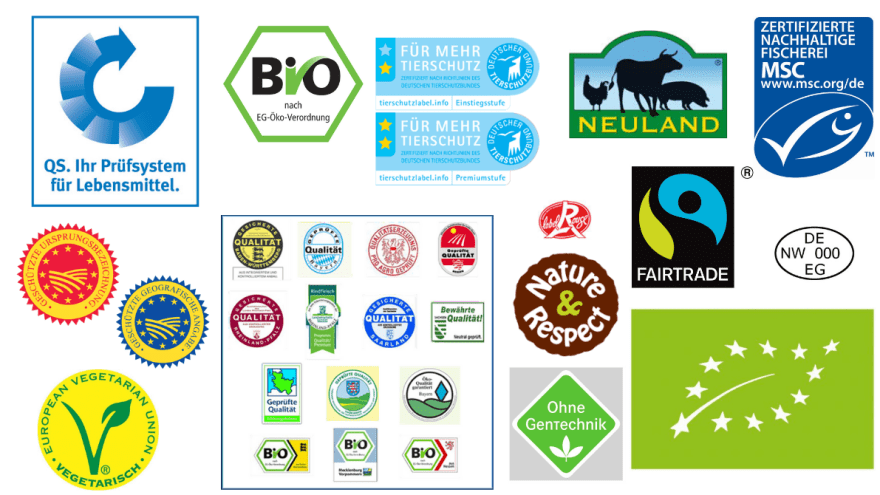
\includegraphics[width=\linewidth]{figures/Siegel Lebensmittel.png}
  \caption{A selection of the many labels printed on German supermarket items}
  \label{fig:labels}
\end{minipage}
\hspace{1cm}
\begin{minipage}{.45\textwidth}
  \centering
   \includesvg[width=0.75\textwidth]{figures/eco_stars.svg}
  \caption{The EU organic logo indicates that a product satisfies the EU Council Regulation on Organic Agriculture}
  \label{fig:eu_organic}
\end{minipage}
\end{figure}



%% ==============
\section{Approaching the Business Case}
\label{sec:approach}
%% ==============
After having decided on building an object detection model to recognize labels on supermarket items, we discussed how to best collaborate in order to develop our computer vision solution. Generally speaking, we agreed on a sprint-like collaboration. This means that each week we had (at least) one meeting with all team members in which tasks were assigned to each team member and the progress since the last week was discussed. The meeting was led by the product owner who was responsible for having a "high-level vision" for the week and made sure everyone was able of doing their tasks and that potential bottle-necks were addressed. The product-owner role was taken by another team member each week. 

After having established our mode of collaboration, we started with collecting and preparing our data. This will be described in greater detail in section \ref{sec:data_split}. Simultaneously, we already started thinking about which model could fit our use case. Which model we chose and the training process will be explained in section \ref{sec:choosing} and section \ref{sec:training}. The results of our model evaluation will be presented in section \ref{sec:evaluation}. In a final step, we deployed our model to the Jetson Nano and integrated it into a front-end to make it accessible for our future users. This final step will be described in greater detail in section \ref{sec:deploy_frontend}.

\newpage
%% ===========================
\section{Creating the Training and Test Data Set}
\label{sec:data_split}
%% ===========================
This section outlines our process of creating a robust dataset for training and testing our model. We detail our data collection methodology, labeling approach, and data augmentation techniques to ensure a diverse and representative dataset for optimal model performance.
%% ===========================
\subsection{Collecting Data}
\label{subsec:collecting_data}
%% ===========================
We first researched whether there were any publicly available datasets that suited our use-case but did not find any. We therefore decided that it was necessary to collect and label the data ourselves. One major benefit of our use-case is that it is quite easy to obtain training data of supermarket items with labels. We did this by simply going to supermarkets and taking photos of items. 

Specifically, we went to two supermarkets, the Edeka in the Scheck-In Center as well as the Lidl at Tivoli. In both supermarkets we took images of different supermarket items. In total we took about 400 photos. When taking the photos we made sure that we also have some negative samples (images containing no label). This resulted in a diverse dataset of approximately 400 images, including both labeled products and negative samples, providing a solid foundation for our model training and evaluation.

%% ===========================
\subsection{Labeling Data}
\label{ch:Foundations:sec:Section2}
%% ===========================
After taking the photos we started labeling them. As we split this task across different students, ensuring labeling consistency between everyone was a central concern for us. \\
We did this in different ways. First, we defined some labeling rules that explained how to deal with edge cases. Some of these label rules are:
\begin{itemize}
  \item If a label is not completely within the image, label the visible part of the image only if at least 50\% of the label are visible.
  \item If the entire label is in the image but is partly visible, then draw a bounding box as large as if the label was not occluded if at least 50\% of the label are visible.
  \item Always draw a bounding box as the smallest possible bounding box that still covers the entire label (all details of the label need to be inside of bounding box).
\end{itemize}

We decided to only label official labels, meaning that our model can not recognize unofficial labels. Therefore, if labels are not recognized, our users can expect that the labels are not official ones/ have no profound meaning. We also decided to exclude labels from foreign countries as well as certain labels that occurred only rarely.

To label the images according to our labeling rules, we used the python library LabelImg (https://github.com/HumanSignal/labelImg). As different people worked simultaneously on the labelling, we always made sure to provide the most recent version of our "classes.txt" on GitLab. Furthermore, we kept a "labelling dictionary" on GitLab where all labels that had been labeled were noted down with an exemplary image and the corresponding class name.
This approach allowed us to quickly label all our data without any conflicts.
%% ===========================


%% ==============
\subsection{Splitting and Augmenting Data}
\label{ch:Foundations:sec:Section2}

 After collecting and labeling our dataset, we implemented a data splitting and augmentation strategy to optimize our training data and improve the robustness of our model.
In the model tuning phase, a ratio of 70\% training data to 15\% validation and 15\% test data on the original images was chosen to build the train-test process. For final training, to achieve the best performance, 85\% of data are applied to train the model, and 15\% are used for validation.

After the train-test splitting, data augmentation was applied only to the training and validation dataset.
The order of these operations was carefully considered: If augmentation was performed first and then split, the test dataset could contain similar augmented images whose originals are in the training dataset. This would lead to data leakage.

The argumentation process involved two main steps: resizing the images and applying various augmentation techniques. To ensure consistency in our dataset and to meet the input requirements of our chosen model, we first implemented an image resizing step. The resizing process was implemented using OpenCV library. We created a Python script that resizes all images in our dataset to a uniform size of 960x960 pixels. This size was chosen to balance between preserving image details and computational efficiency.

Following the resizing process, we implemented a comprehensive data augmentation strategy to increase the diversity of our training data. We utilized the Albumentations library, a popular Python package for image augmentation in machine learning tasks. Our augmentation pipeline consists of several transformation strategies, each designed to simulate different real-world scenarios our model might encounter.

Our augmentation pipeline includes the following strategies:

\begin{enumerate}
    \item Rotation and Color Adjustment:
    \begin{itemize}
        \item Safe rotation up to 180 degrees
        \item Color jittering (brightness, contrast, saturation, and hue adjustments)
    \end{itemize}
    
    \item Brightness/Contrast Adjustment and Cropping:
    \begin{itemize}
        \item Random brightness and contrast changes
        \item Random sized bounding box safe crop
    \end{itemize}
    
    \item Horizontal Flipping and Blurring:
    \begin{itemize}
        \item Horizontal flip
        \item Gaussian blur
    \end{itemize}
    
    \item Vertical Flipping and Elastic Transform:
    \begin{itemize}
        \item Vertical flip
        \item Elastic transform
    \end{itemize}
\end{enumerate}


For images with bounding box annotations, we ensured that the augmentations were applied to both the image and its corresponding bounding boxes. This was achieved by using Albumentations' BboxParams with the YOLO format. We also set a minimum visibility threshold of 0.5 for bounding boxes to ensure that heavily cropped or transformed objects were not included in the augmented dataset.

For images without bounding boxes (our negative samples), we applied similar augmentations but without the bounding box transformations.

Each strategy is applied to every image in our dataset, resulting in four additional augmented images per original image. This process effectively quintuples the size of our dataset.
\begin{figure}[ht]
\begin{minipage}{.46\textwidth}
  \centering
  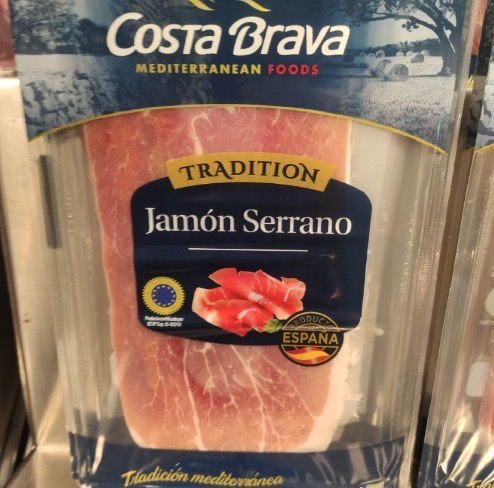
\includegraphics[width=\linewidth]{figures/argutmented_2.jpg}
  \label{fig:costa_brava_original}
\end{minipage}
\begin{minipage}{.5\textwidth}  \centering
  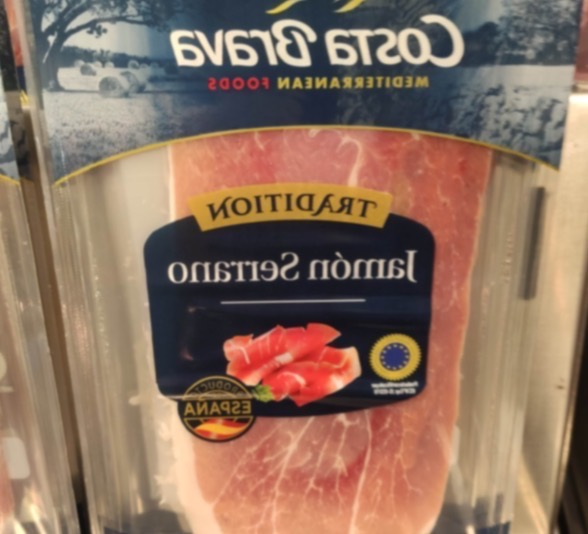
\includegraphics[width=\linewidth]{figures/argumented_1.jpg}
  \label{fig:costa_brava_augmented}
\end{minipage}
\caption{With HorizontalFlip and GaussianBlur operations augmented image}
\label{fig:costa_brava_comparison}
\end{figure}

The augmentation process was automated using a Python script that iterates through all images in the input directory, applies the augmentations, and saves the resulting images and updated annotation files in an output directory. This approach allowed us to efficiently process our entire dataset and generate a comprehensive augmented dataset for training.

By implementing this data preparation and augmentation strategy, we aimed to improve our model's ability to detect labels under various conditions. The combination of consistent image sizing and diverse augmentations contributes to a more robust and generalizable model for detecting labels on supermarket items. Specifically:

\begin{itemize}
    \item Rotations and flips help the model recognize labels in different orientations.
    \item Color adjustments and brightness/contrast changes simulate various lighting conditions.
    \item Cropping and elastic transformations mimic different viewing distances and label deformations.
    \item Blurring prepares the model for slightly out-of-focus images.
\end{itemize}

These augmentations collectively enhance the model's ability to handle real-world variations in label appearance, positioning, and imaging conditions, leading to improved performance in diverse supermarket environments. Upon completion of the augmentation process, both the augmented and original images, along with their corresponding bounding box text files, were prepared for training. This allowed us to create a comprehensive and diverse training set that included both the original and artificially expanded data.

It is important to emphasize that the augmentation process was iterative. After each training run, we carefully evaluated the model's performance and adjusted our augmentation strategies accordingly. For instance, in our first version of color jittering, we found that some of the augmented images were too distorted, leading to a degradation in model performance.



\newpage
%% ===========================

\section{Choosing an Object Detection Model}
\label{sec:choosing}
%% ==============
When selecting an object detection model for the project, we considered several critical factors. First and foremost, the model needed to be state-of-the-art, ensuring that it could leverage the latest advancements in computer vision to deliver high accuracy and reliability. \\
Given the hardware constraints of the Jetson Nano, our chosen model also had to maintain a high frame per second (FPS) rate to facilitate real-time processing capabilities. Robustness was another crucial criterion, as the model must perform consistently across a variety of conditions and environments without significant degradation in performance. \\
After thorough evaluation, we chose YOLOv4-tiny as our preferred model. YOLOv4-tiny is a streamlined version of YOLOv4, specifically designed to operate efficiently on resource-constrained devices like the Jetson Nano while still delivering impressive performance. \\
Compared to YOLOv4, which offers better accuracy and detection capabilities due to its more complex architecture and size, YOLOv4-tiny sacrifices some precision for speed and efficiency, making it an ideal choice for our case. \\
The comparison of YOLOv4-tiny to other models can be observed in the following graph.

\begin{figure}[ht]
    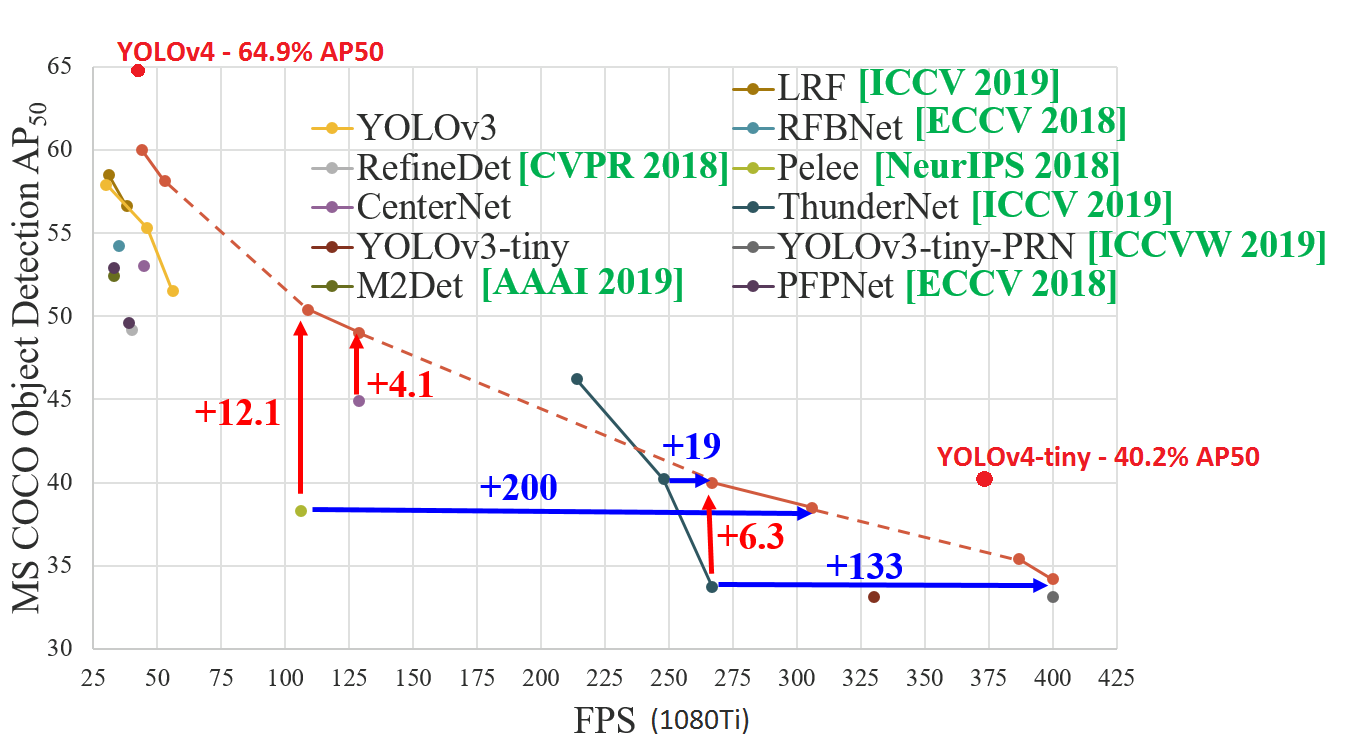
\includegraphics[width=\textwidth]{figures/yolov4-comparison.png}
    \caption{Comparison of different models for object detection}
    \label{fig:model_comparison}
\end{figure}

\newpage 
%% ==================
\section{Training Darknet}
\label{sec:training}
%% ==================
To train and evaluate our model, we chose the Darknet framework due to its flexibility and support for state-of-the-art neural networks like YOLOv4-tiny. Darknet is an open-source neural network framework written in C and CUDA. It is known for its speed and efficiency, particularly in object detection tasks. This framework provides a straightforward setup for training and deploying models, with a configuration system that allows for easy adjustments of network architecture and hyperparameters. Additionally, Darknet supports GPU acceleration, which significantly speeds up both training and inference processes, making it an excellent choice for our performance-sensitive application.

\subsection{Compiling Darknet}
To compile Darknet on the Jetson Nano, it is essential to have OpenCV support. However, the default OpenCV installation on the Jetson Nano does not include CUDA or GStreamer support, which are critical for our application. CUDA support is necessary for GPU acceleration, while GStreamer is required to access the CSI camera that comes with the Jetson Nano. Therefore, we had to compile OpenCV ourselves, ensuring it included both CUDA and GStreamer support.

The process of building the complete OpenCV package is resource-intensive, requiring more than 4 GB of RAM. The Jetson Nano, with its 2 GB of RAM and 2 GB of zram swap space, lacks sufficient memory for this task. To overcome this limitation, we temporarily installed dphys-swapfile to extend the swap space using the SD card. This temporary measure provided the additional room needed for compilation. After successfully building OpenCV, we removed dphys-swapfile to eliminate the reliance on SD card swapping, which can wear out the SD card and reduce system performance.

Once OpenCV was successfully compiled with the necessary support, we proceeded to compile Darknet on the Jetson Nano, integrating it with the customized OpenCV installation.

\subsection{Training Process}
While inference is conducted on the Jetson Nano, training the model required more computational power than the Jetson Nano could not provide. Therefore, we performed the training on a separate device equipped with an NVIDIA RTX 4090 GPU. This high-performance GPU significantly reduced the training time, allowing us to iterate quickly on our model. Compiling Darknet on the RTX 4090-equipped device was straightforward compared to the Jetson Nano, mainly due to the more powerful hardware and the absence of memory constraints.

\subsection{YOLOv4-tiny Configuration}
The specifics about the configuration file we created for our model can be found in the appendix (\ref{app:config_file}). Such a configuration file is robust to changes, meaning a change of number of classes only requires the end user to modify the number of filters of the convolutional layers just before each YOLO layer. Since YOLOv3 and above detects 3 boxes per grid cell, the number of required filters for the convolutional layers can be found with the following formula: $ \text{filters} = (\text{classes} + 5) \times 3 $.

\newpage 
%% ==================
\section{Evaluating Darknet}
\label{sec:evaluation}
%% ==================
After training the model the next step was to evaluate the model’s performance. Here, we focused on the “Average Precision” (AP) metric, as it accounts for both precision and recall by combining the two of them into one metric. This is highly important for us, because solely focusing on precision would cause our model to only detect the label of easily detectable majority classes, ignoring any minority classes. Furthermore, a pure focus on recall would also be a disadvantage, as it would cause the model to predict way more bounding boxes, than there actually are, just in order to not miss any of these actually existing bounding boxes.

Overall, the model evaluation was part of an iterative process of augmenting images, training and testing that helped in three ways:
(1) to improve our augmentation strategies, (2) to serve as a starting point for further performance enhancing ideas and (3) to provide an understanding of the object detection quality of our final model.

In the more exploratory process of (1) improving our augmentation strategies and (2) generating further ideas to enhance the model, we used augmented data in both the training and testing, to be able to work with a larger dataset. However, in (3) the final evaluation of our model we made sure to only test on real images that did not have any augmented images associated to them as described in \ref{sec:data_split}.  In the following subsections we will take a closer look at each of these three areas of our model evaluation.
%% ==================
\subsection{Improving our augmentation strategies}
%% ==================

As described in the augmentation process the whole cycle of augmentation, training and testing was iterative and new test results revealed insights on what kind of data augmentation strategies were useful and which ones had to be adopted. After each change in our augmentation pipeline, we checked how performance was influenced and investigated the occurrence of poor performing classes. By doing so, we were able to detect and adopt augmentation steps, that were (differently from what we expected) not contributing towards a better generalization and training, but rather leading to unrealistic distortions of augmented images. 

%% ==================
\subsection{Informing further performance enhancing ideas}
%% ==================

Another way in which the continuous evaluation of model performance throughout our project helped us, was that it served as a starting point for further performance enhancing ideas. More specifically when looking at our original results \ref{fig:ap_unmerged} one can witness, that the worst performing class is the “nutriscore\_d” with an AP score below 40\%. Whilst the other “nutriscore” labels seem to be more easily detected, the “nutriscore\_c” and “nutriscore\_a” labels still have some room for improvement. 

\begin{figure}[H]
    \centering
    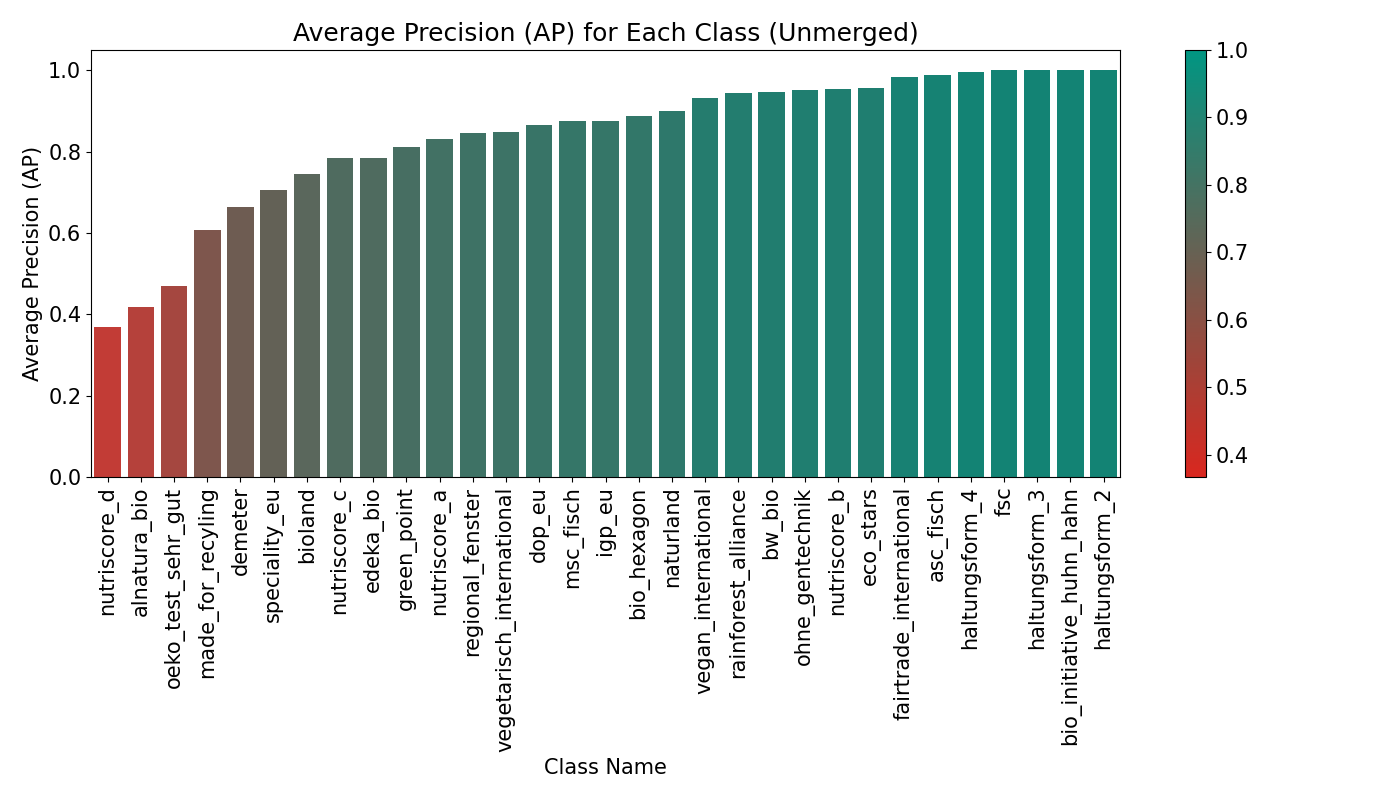
\includegraphics[width=1\linewidth]{Average_Precision_AP_for_Each_Class_Unmerged.png}
    \caption{Average Precision for each class}
    \label{fig:ap_unmerged}
\end{figure}

When thinking about it, this makes sense, as these labels all look relatively similar and telling them apart appears to be a difficult job for the model. Thus, we refocused on a user-centric view and asked ourselves, what the user is interested in. For the user it is most important (1) to trust the model and its predictions and (2) to be displayed the correct information for a label, thus informing his product choice. In the case of the “nutriscore”, understanding what e.g. “nutriscore\_a” means requires understanding the general concept of the “nutriscore” first. This means that the “nutriscore” as a concept must be explained in any case, regardless of what specific “nutriscore” is detected. Therefore, we found that we could try to combine the multiple “nutriscore” labels into one class “nutriscore” and check whether the AP score would improve for this class. 

\begin{figure}[H]
    \centering
    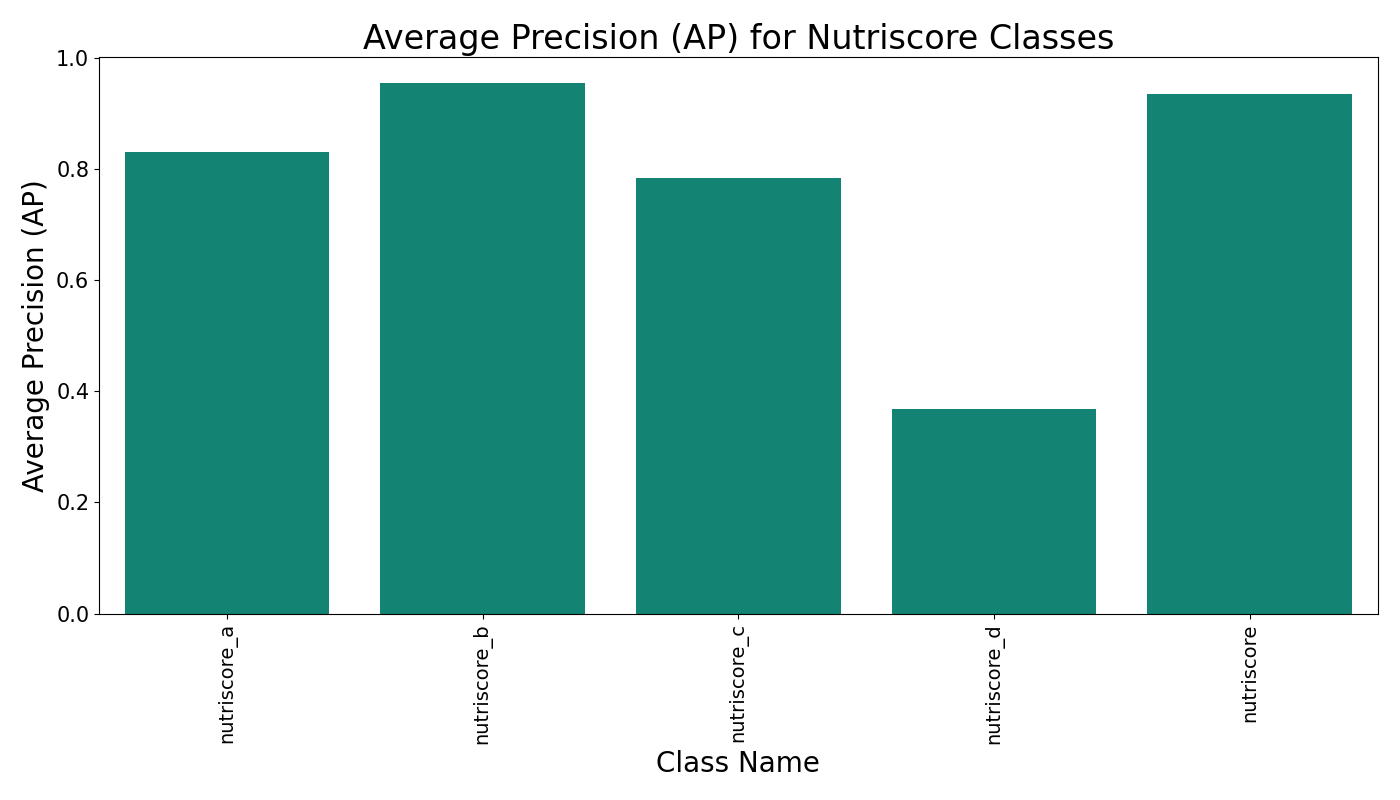
\includegraphics[width=1\linewidth]{Average_Precision_AP_for_Nutriscore_Classes_presentation.png}
    \caption{AP for single and merged "nutriscore" classes}
    \label{fig:ap_nutriscore}
\end{figure}

As can be seen in Figure \ref{fig:ap_nutriscore}, in fact the AP score for the class “nutriscore”, which contains the merged individual classes, has a much higher score than the mean of the AP scores of the individual classes. This allows us to satisfy the user needs by (1) providing a more robust label detection and thus being able to (2) provide adequate information for this label. However, this comes at the expense of providing information specific to the actual “nutriscore” class (e.g. “a”), but this might be acceptable as firstly, a general explanation of the “nutriscore” has to be provided anyway and secondly, it is better to  display correct general information then incorrect specific information. However, being able to detect each “nutriscore” individually remains an interesting endeavor for future work.

Out of curiosity, and to maintain consistency we also merged the classes of the “haltungsform” labels, with some interesting findings. As the original AP scores of the individual “haltungsform” labels were already high with an AP score of above 90\%, we were interested in how the performance of the merged classes would change. 

\begin{figure}[H]
    \centering
    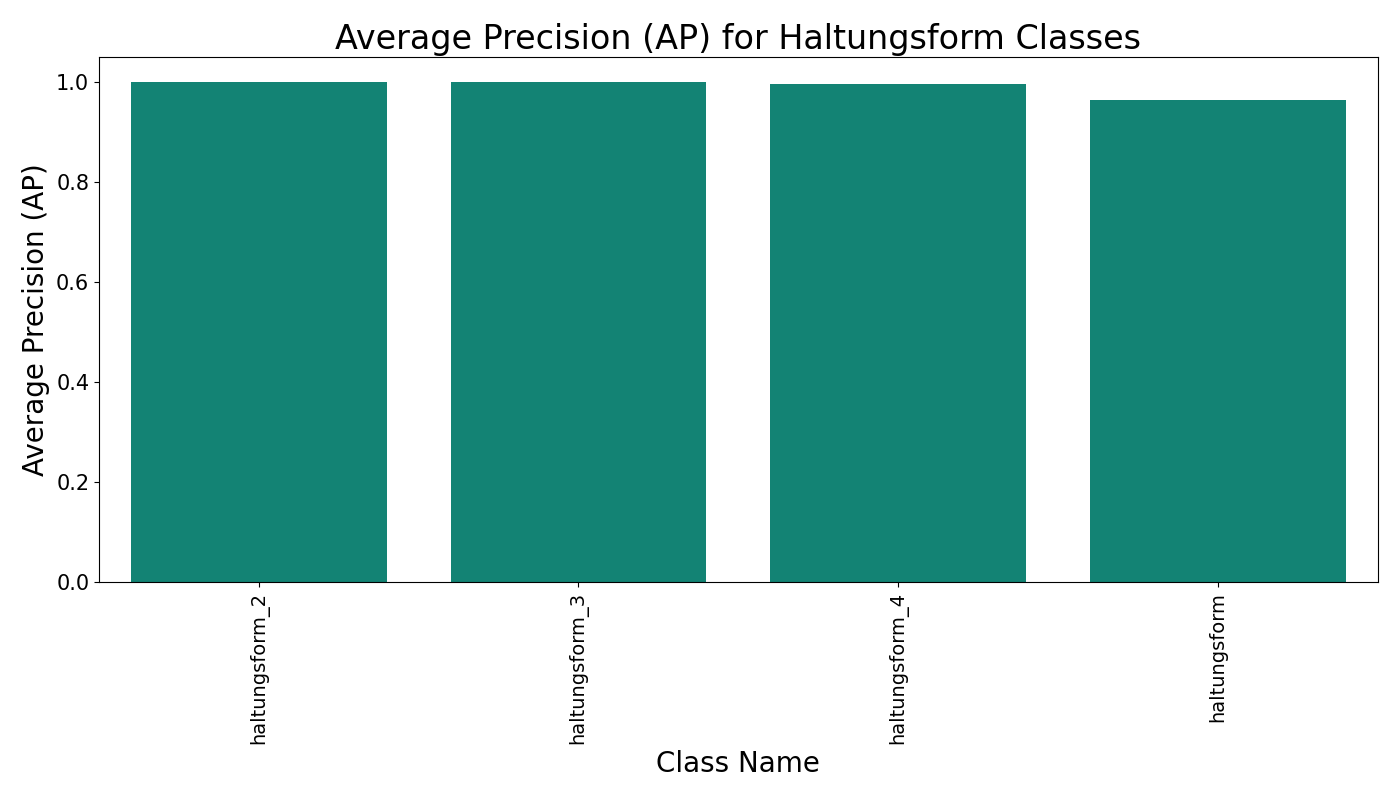
\includegraphics[width=1\linewidth]{Average_Precision_AP_for_Haltungsform_Classes_presentation.png}
    \caption{AP for single and merged "haltungsform" classes}
    \label{fig:ap_haltungsform}
\end{figure}

As can be seen in Figure \ref{fig:ap_haltungsform}  the performance remained relatively unchanged, with even a small decrease in the AP score, but well above an AP score of 90\%. To maintain a consistent approach and to be more robust towards detecting “haltungsform\_1” labels, that were neither in the training set nor in the testing set, we decided to keep the merged “haltungsform” label in our final model. The resulting performance for all classes including the merged classes “nutriscore” and “haltungsform” can be seen in Figure \ref{fig:ap_merged}.

\begin{figure}[H]
    \centering
    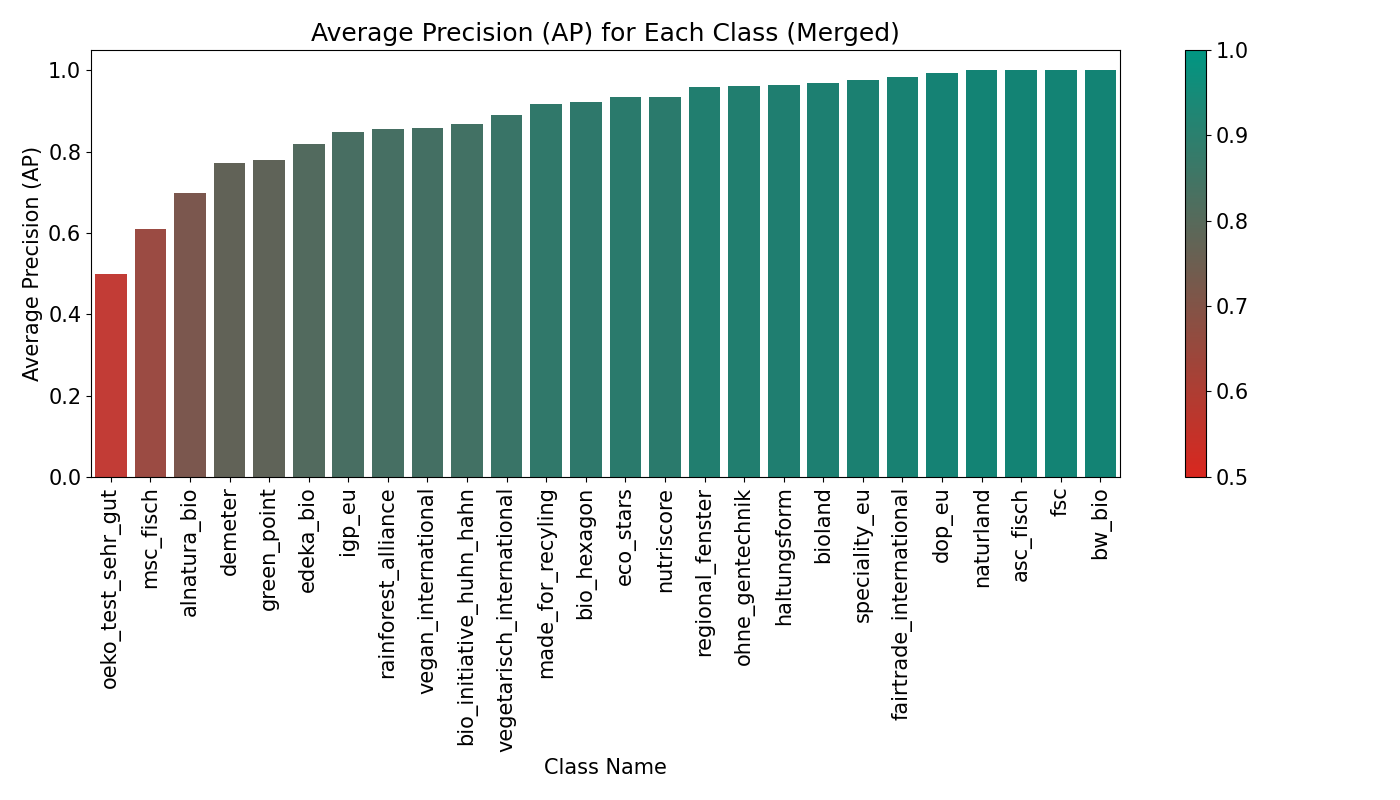
\includegraphics[width=1\linewidth]{Average_Precision_AP_for_Each_Class_Merged.png}
    \caption{Average Precision for each class (merged)}
    \label{fig:ap_merged}
\end{figure}
 
%% ==================
\subsection{Evaluation}
%% ==================

The third and most straightforward way in which the evaluation of our model creates value is by providing insights into the object detection quality of our final model. Whilst our very final model used for deployment was trained on all available data, we made sure to have a clean evaluation beforehand using a train test set that was generated as described in the section \ref{sec:data_split}. The evaluation results of our final model are depicted in Figure \ref{fig:ap_final}. 

\begin{figure}[H]
    \centering
    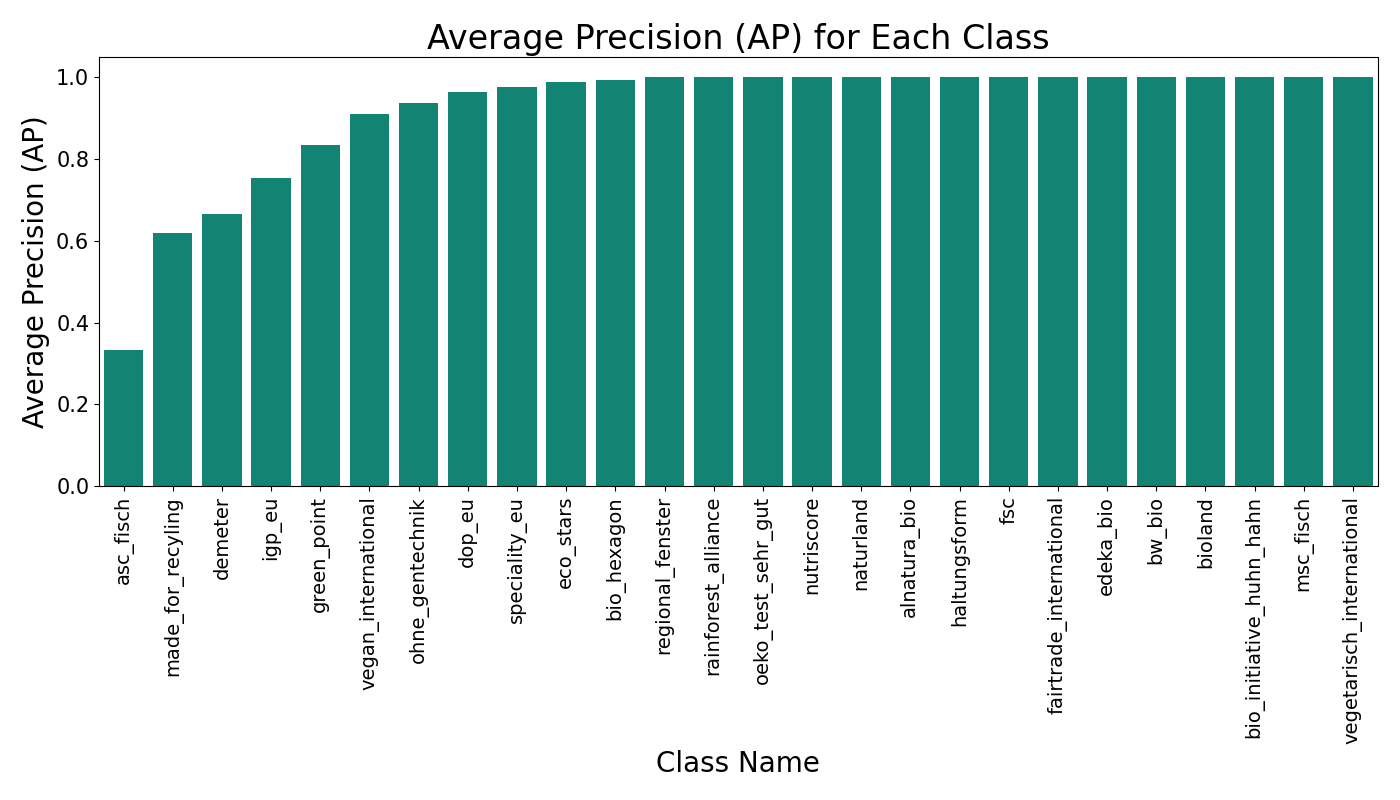
\includegraphics[width=1\linewidth]{Average_Precision_AP_for_Each_Class_presentation.png}
    \caption{Average Precision for each class - final model}
    \label{fig:ap_final}
\end{figure}

First, it can be seen that overall, most classes achieve very high AP scores, resulting in an “Mean Average Precision” (mAP) across all classes of 92.2\%. 

Next, we want to look at the “Intersection over Union” (IoU), which depicts the accuracy of the predicted bounding boxes by measuring the overlap between a predicted bounding box and the ground truth bounding box. Here we have an IoU score of 74.06\%, which means that 74.06\% of the original bounding box area aligns with the predicted bounding boxes.

Finally, we also want to consider how many of our 214 actual bounding boxes in the test set were detected correctly (True Positives), how often a bounding box was predicted that did not actually exist (False Positives) and how often an actually existing bounding box was not detected (False Negatives). These results are depicted in Figure \ref{fig:cm_final}. Note, that in a multi class object detection task, there are no True Negatives. 

\begin{figure}[H]
    \centering
    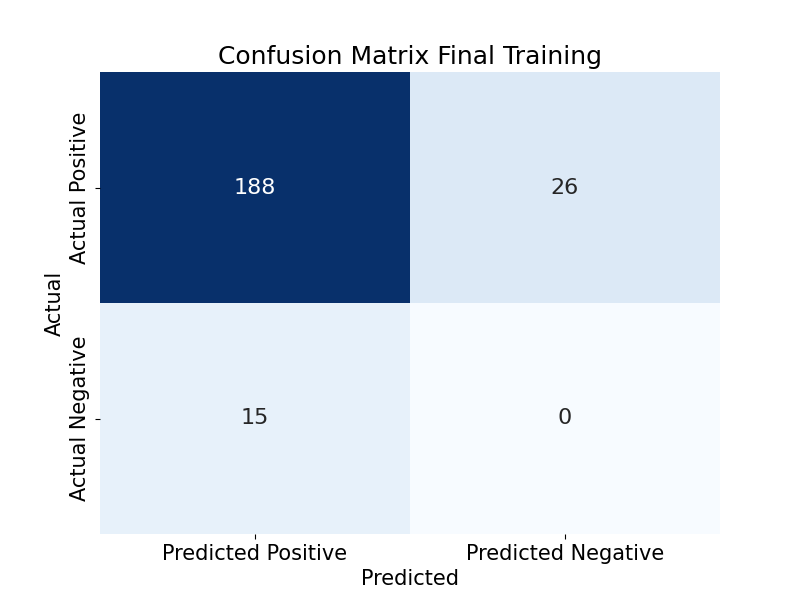
\includegraphics[width=0.75\linewidth]{Confusion_Matrix_Final_Training.png}
    \caption{Confusion Matrix of final model}
    \label{fig:cm_final}
\end{figure}

In Conclusion one can say that our model archives good results for most classes across different metrics. Nevertheless, in future efforts, approaches should be employed to improve the performance of poor performing classes such as the “asc\_fisch” label. One could think about amplifying data augmentation strategies or increasing the data collection for poor performing classes.

\newpage
%% ==================
\section{Putting it all together: our web page}
\label{sec:deploy_frontend}
%% ==================

While it is possible to just view the Darknet output as a video stream including bounding boxes on the Jetson Nano's desktop (see the demo), we wanted to provide a real frontend to showcase what the final product could look like. 
Our program has two modes, image and video, to either take single images and show the detected labels on them or to show a live video feed and update the labels shown as they are detected in it. The frontend is mostly similar for both modes. It contains two columns. The column on the left includes a container in which either still images or the video feed is shown. The column on the right consists of an expanded accordion element, showing the detected labels. There is an accordion item for each detected label, as multiple labels can be detected in a single image or frame at the same time. Each item shows the label's respective icon, name, and a short description. These shown labels are updated live with regards to the currently shown image or frame. Figure \ref{fig:frontend} shows our website in action, detecting the labels for an image.

\begin{figure}[H]
    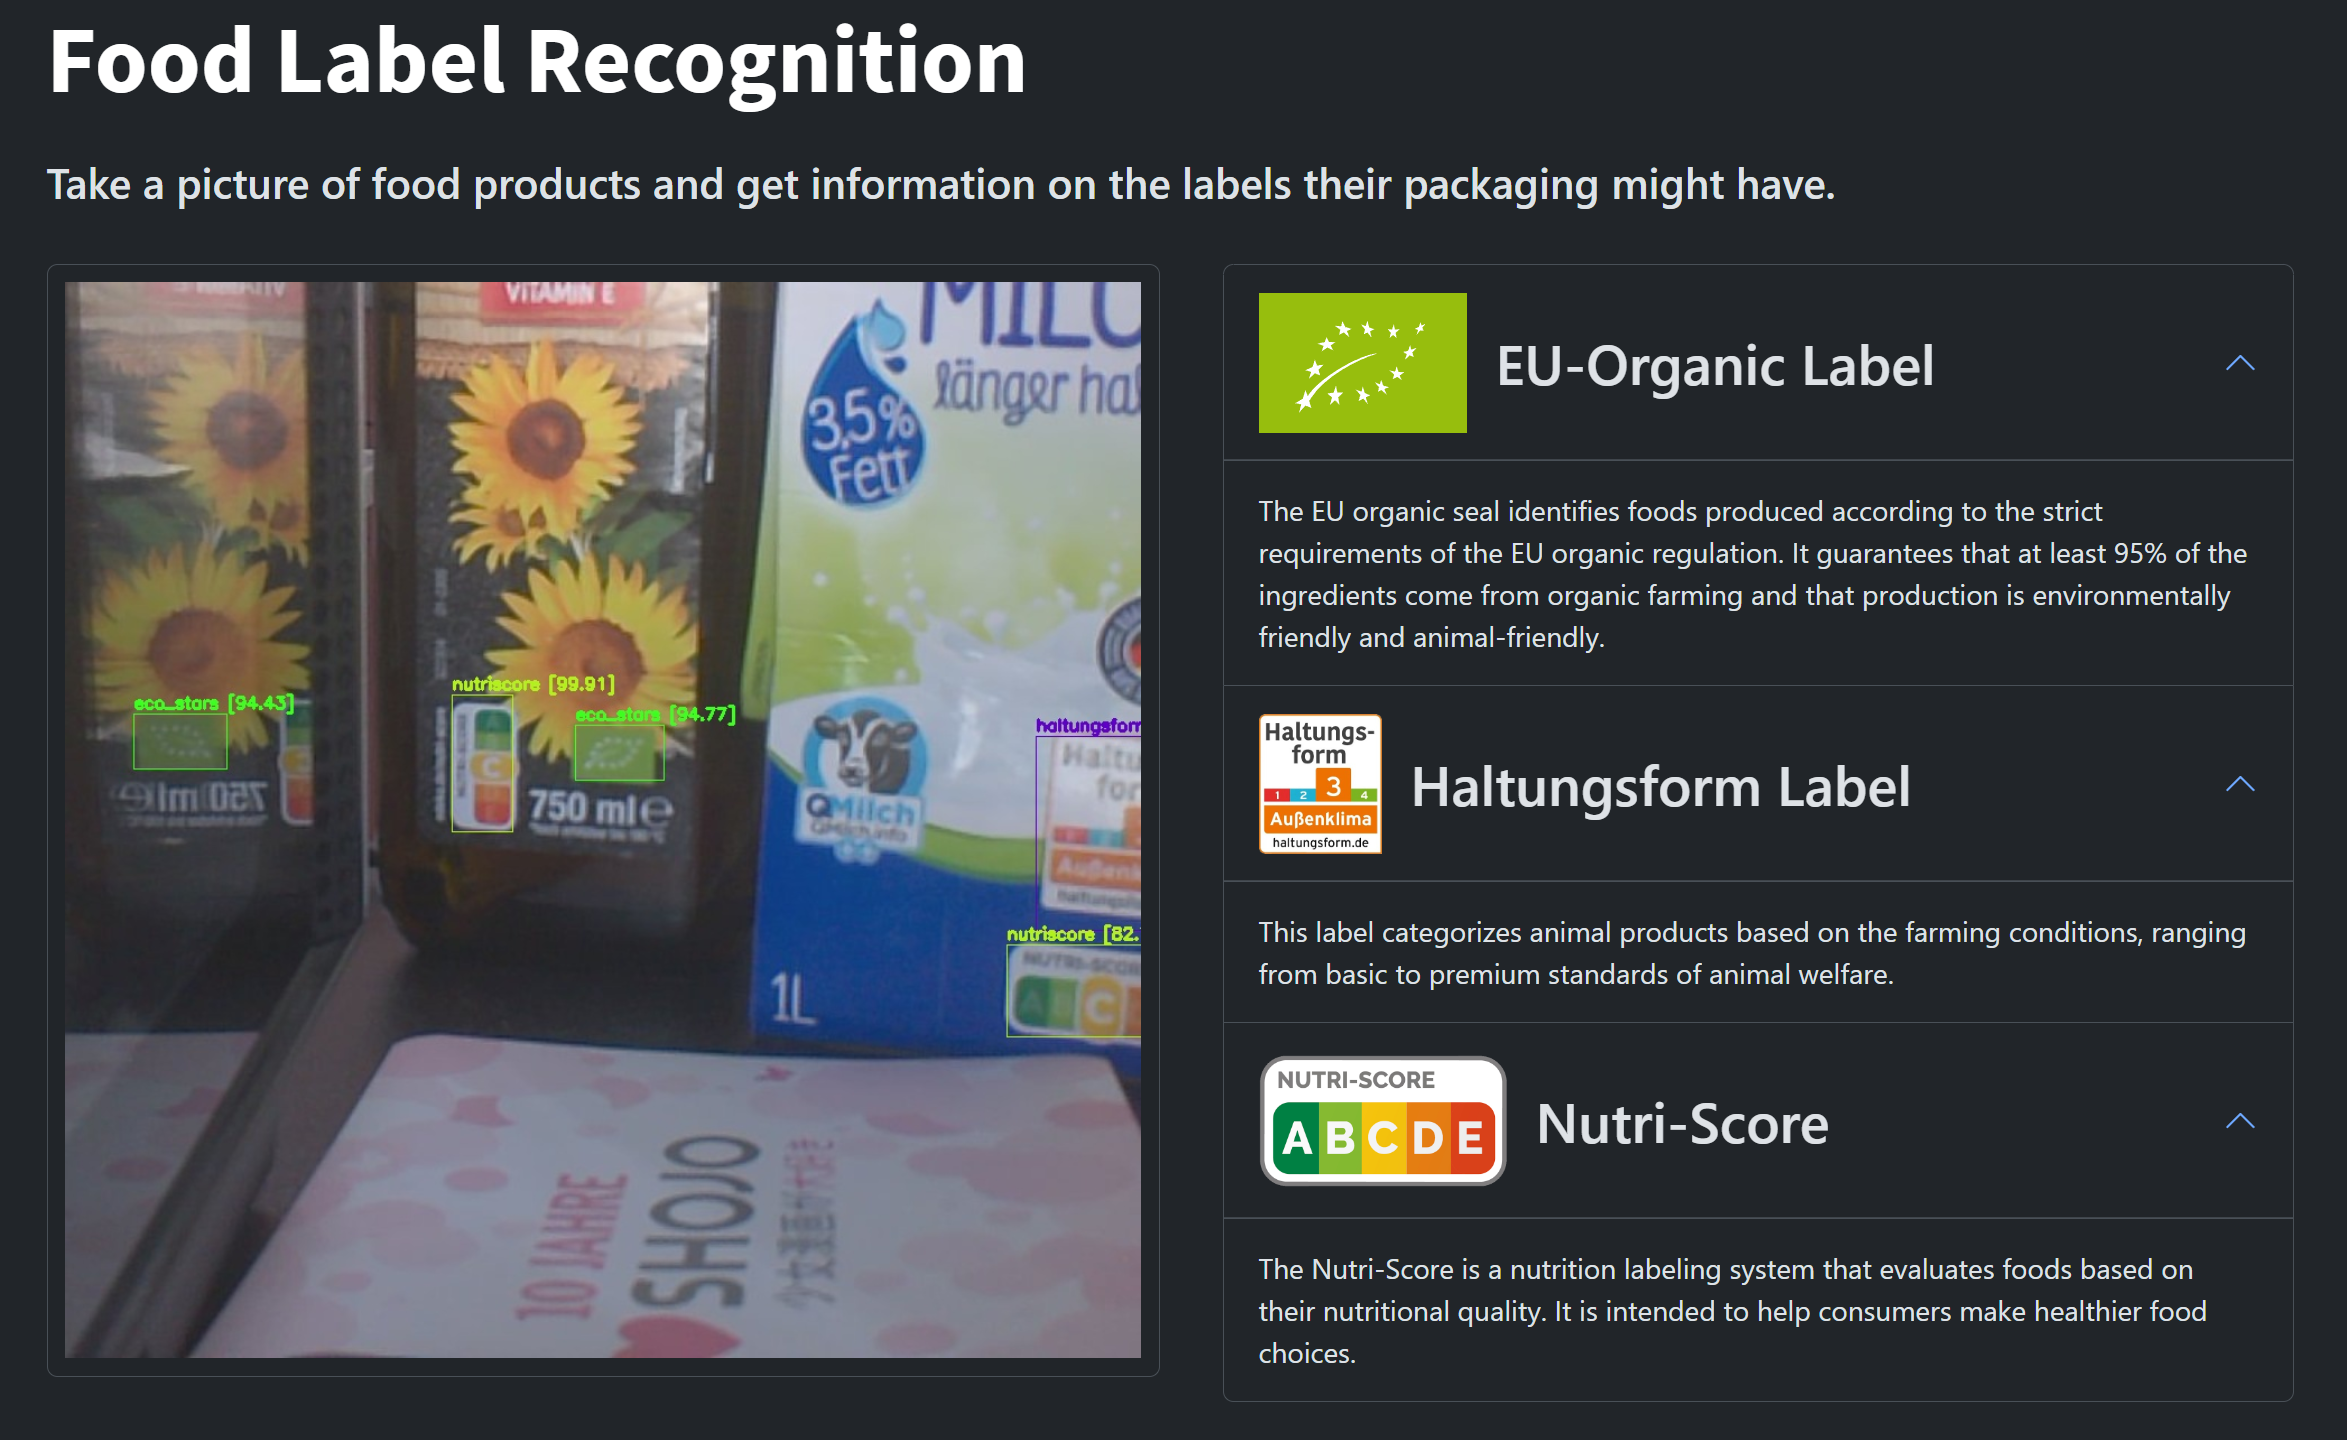
\includegraphics[width=\textwidth]{figures/web_sample_cropped.PNG}
    \caption{Cropped Screenshot of our final website}
    \label{fig:frontend}
\end{figure}

Our original implementation was based on Streamlit, as we wanted to keep our code base predominantly written in python. Furthermore, Streamlit makes it rather simple to design and build the frontend: it is integrated in the backend, as no HTML, CSS or JavaScript is required. However, after some testing we found out, that due to hardware constraints, we would not be able to run Streamlit on the Jetson Nano and therefore had to switch our technology. Also we had at first planned to only include the image-mode. Video-mode would have been considerably more challenging to implement with Streamlit. Figure \ref{fig:program_flow} shows our first Streamlit-based design for the program flow.

\begin{figure}[H]
    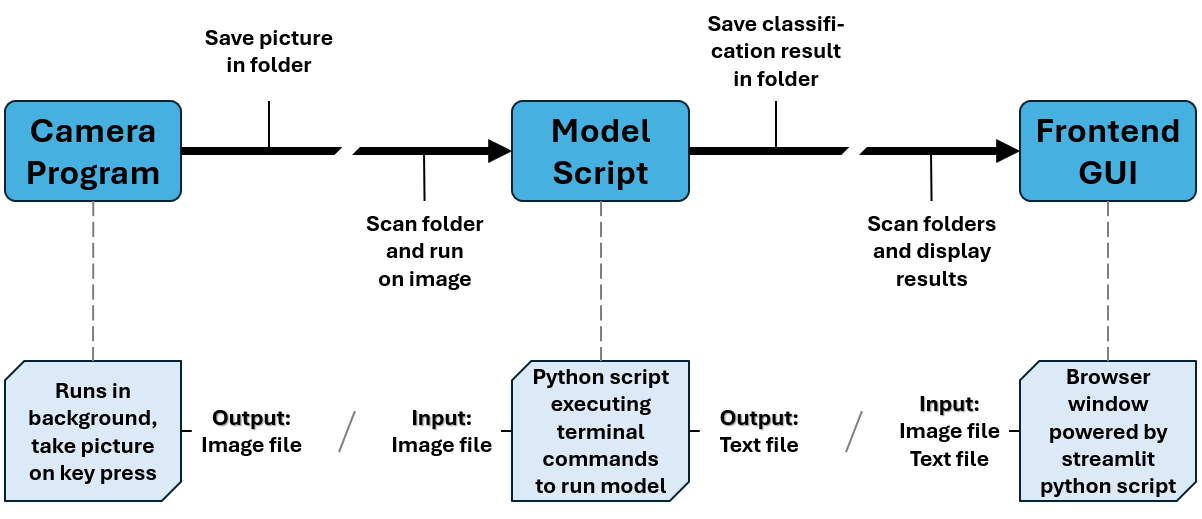
\includegraphics[width=\textwidth]{figures/program_flow.png}
    \caption{Original diagram of our components, their tasks, and interfaces for the single image mode}
    \label{fig:program_flow}
\end{figure}

We then switched to a more traditional approach, consisting of a separate frontend and backend. This time we deliberately tried to include as few frameworks and packages as possible. As a result, we chose the very lightweight web framework Flask for our backend. Our frontend is built with HTML, CSS, and plain vanilla Javascript. Again our focus was to first implement the image-mode as a less resource-consuming kind of prototype to the video-mode.

Our final architecture from taking a photo or video to showing the results on the website differs between the image and video mode. With the image mode being implemented first, we chose to rather have the parts separate. our architecture consists of the camera program, which takes photos on the press of a key and saves them individually in a specific directory. The Flask frontend periodically scans this directory for new images and runs our YOLOv4-tiny model on them using Darknet via a Python wrapper. The image is then edited to show the bounding boxes for detected labels and is displayed on the website together with the label information based on the respective detections. 
Originally, we also chose to separate the model from the frontend by running the model periodically in the terminal and saving its detections as a text file the directory of which the frontend would also scan and read together with the latest image. We rejected this approach, because the integration with the frontend in Python is less resource heavy and has fewer points of failure. We also do not really need the modularity provided by this approach for our project. Figure \ref{fig:program_flow_img} shows our design for the final image-mode program flow.

\begin{figure}[H]
    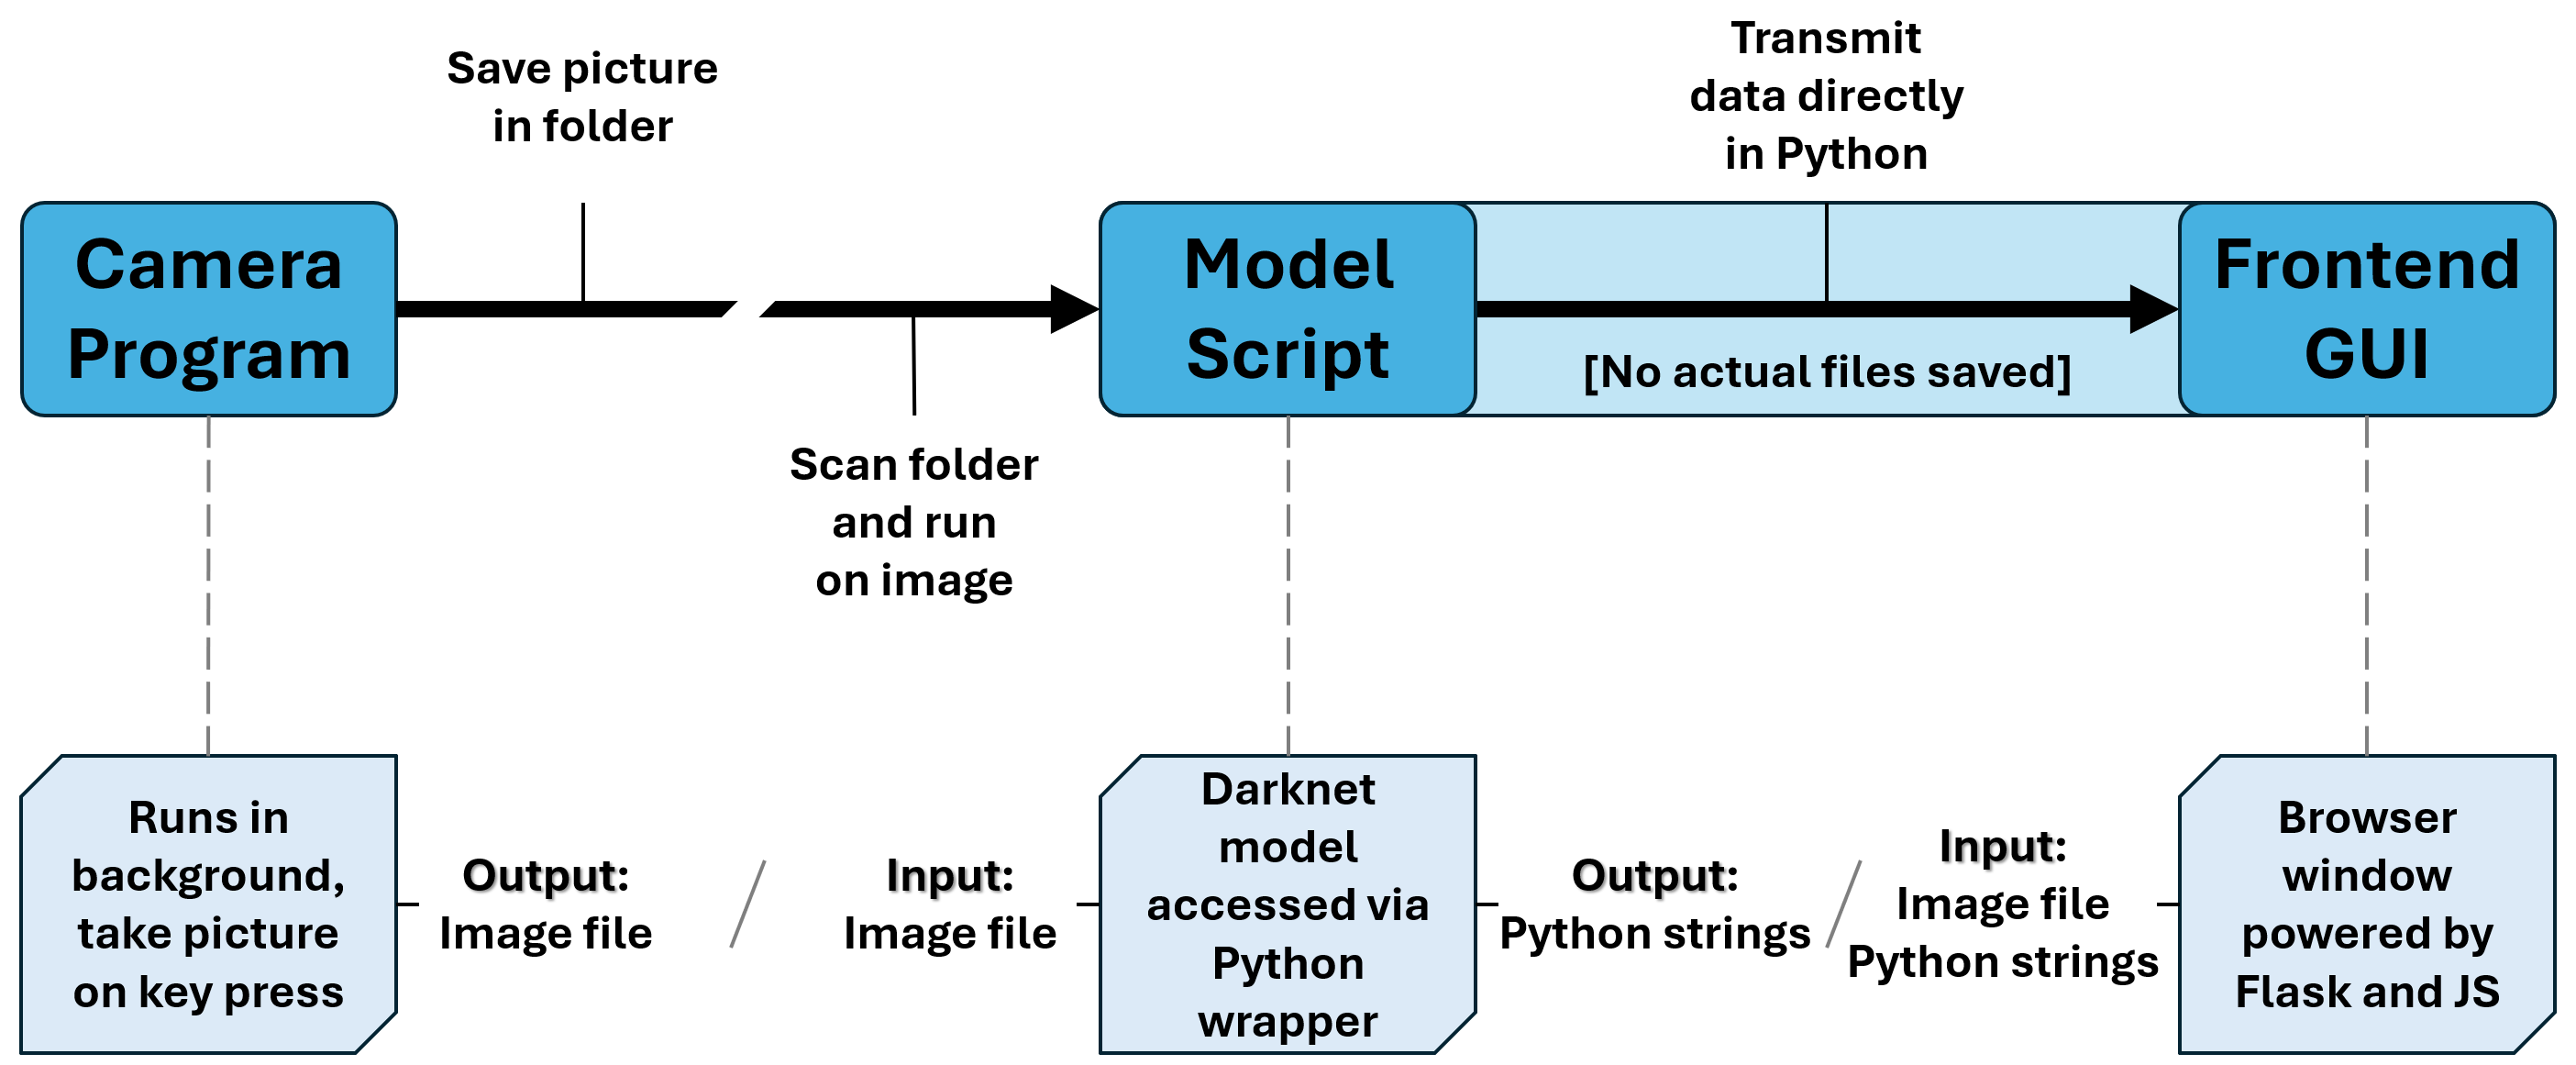
\includegraphics[width=\textwidth]{figures/process_img.png}
    \caption{Diagram of our components, their tasks, and interfaces for the single image mode after switching to Flask}
    \label{fig:program_flow_img}
\end{figure}

For the video mode, we decided on a even more integrated approach. Here, our web server is the central module. Using the OpenCV package with a GStreamer pipeline, it directly controls the camera and reads the video stream from it. This is not only a design decision, but also a practical one due to the real-time properties of live video and the resulting difficulties in first saving or buffering it from one module before accessing it by another. We treat the video as a series of frames, which are individually displayed one after another in the frontend. The YOLOv4-tiny model loaded into Darknet is used via the Python wrapper to detect the labels for the frames. Neither the frames, nor the detected labels are intermediately saved on the hard drive. Once all relevant data for each frame, its bounding boxes, and detected labels is gathered and computed, it is displayed to the user. Because of hardware constraints, we only detect the labels in every 15\textsuperscript{th} frame. The detected labels and bounding boxes are then shown for the next raw frames as well, until a new detection is run. Figure \ref{fig:program_flow_vid} shows our design for the final video-mode program flow.

\begin{figure}[H]
    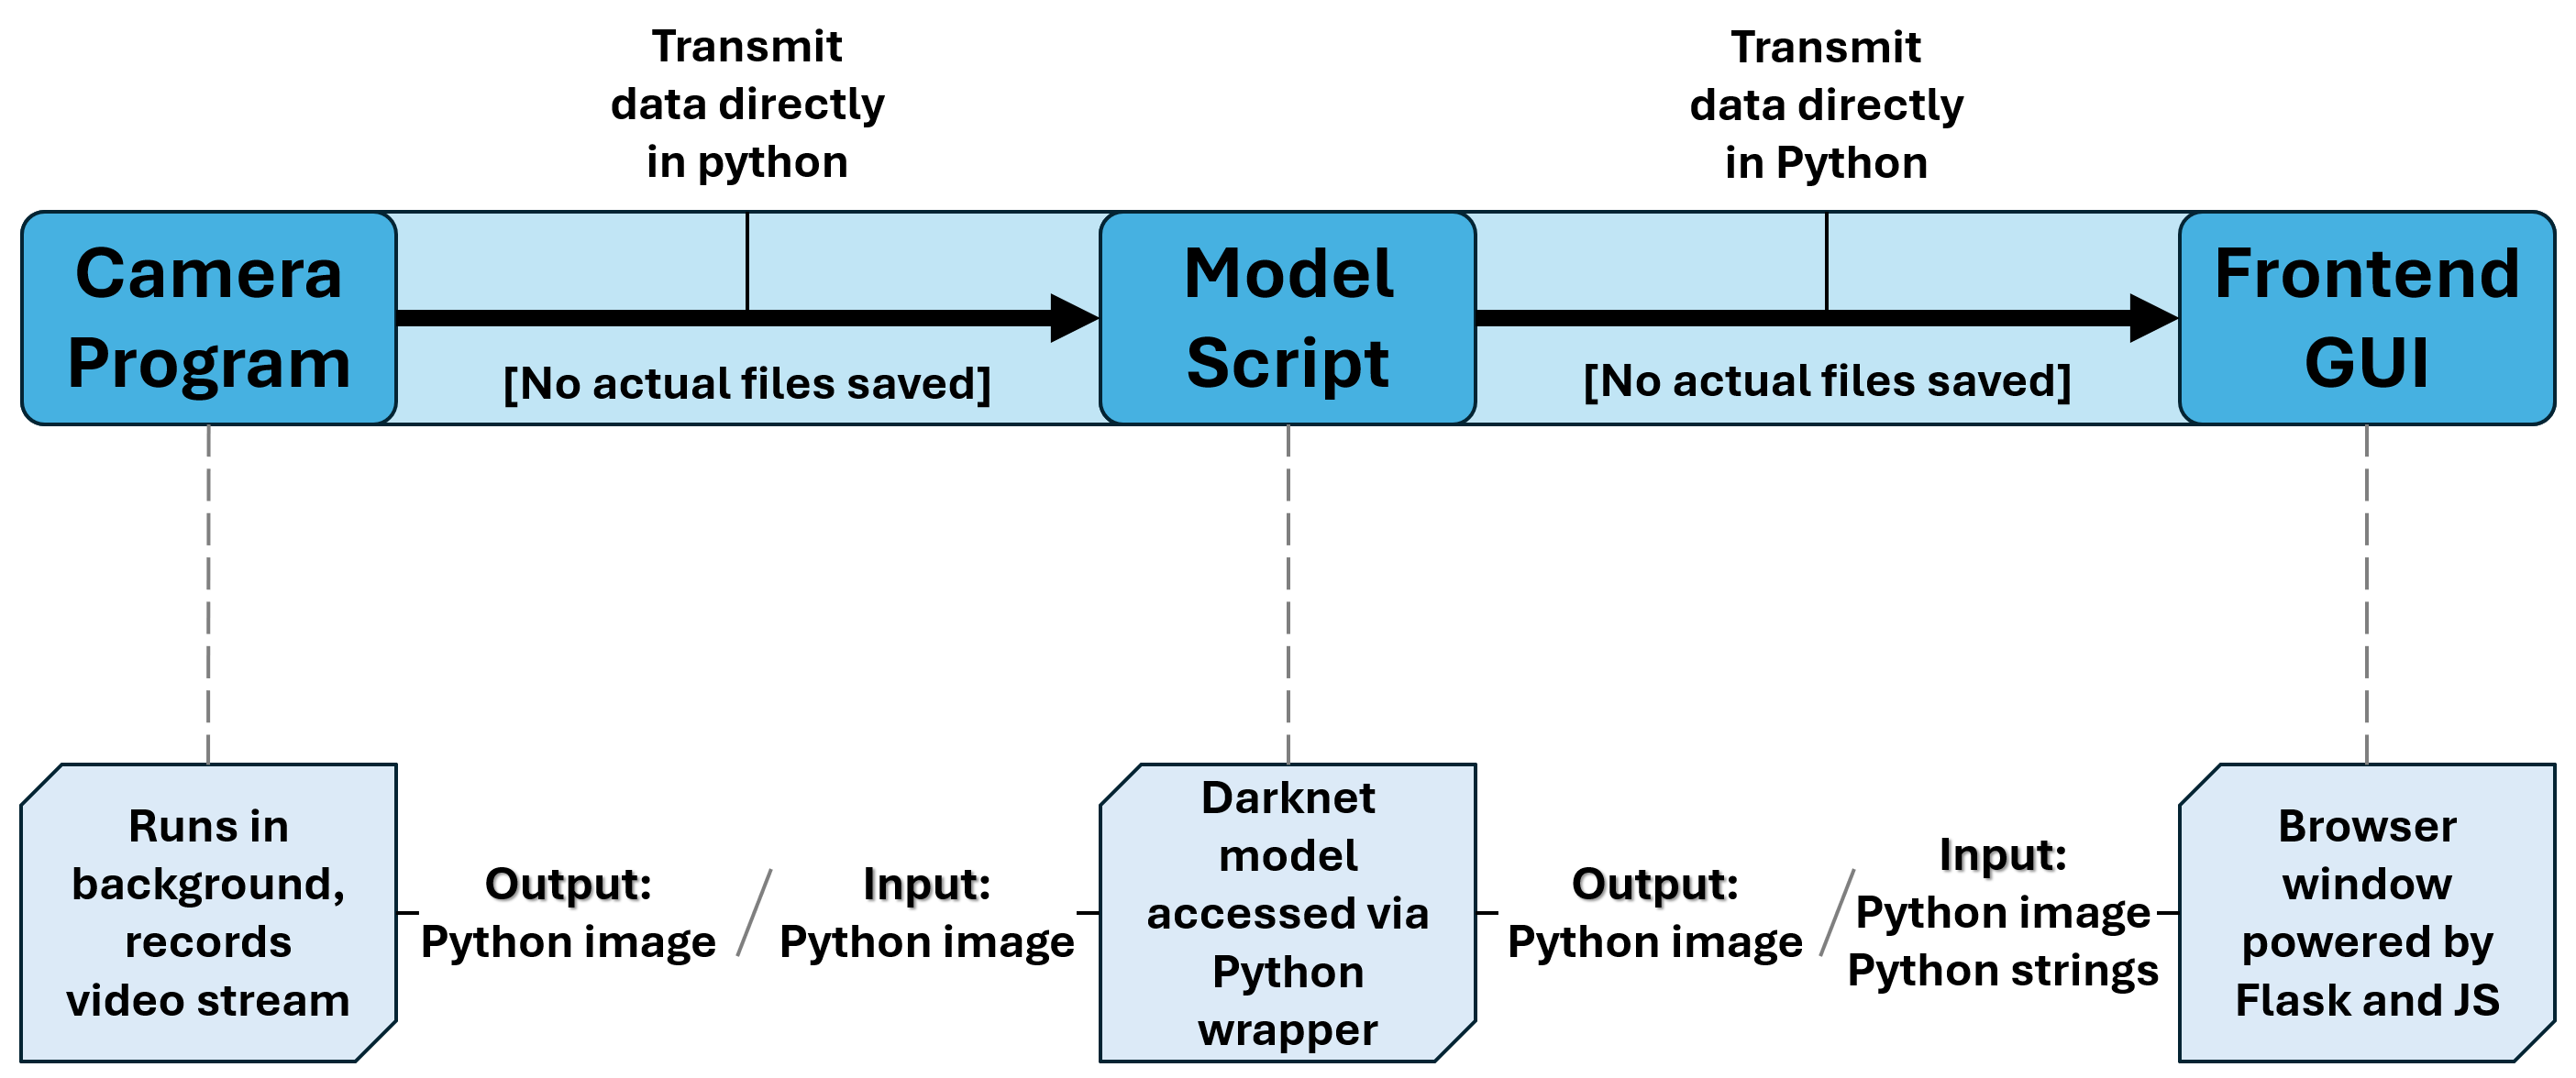
\includegraphics[width=\textwidth]{figures/process_vid.png}
    \caption{Diagram of our components, their tasks, and interfaces for the final live video streaming mode}
    \label{fig:program_flow_vid}
\end{figure}


\subsection{Running the Frontend + Model}
The final runnable program is located in the main folder. The instructions are based on it as the starting directory. All code is expected to be run on the Jetson Nano device.

\subsubsection*{Setup}

Install all packages specified in the \texttt{requirements.txt} file:

\begin{lstlisting}[style=bash]
pip install -r requirements.txt
\end{lstlisting}

Run the following command to install our custom modules:

\begin{lstlisting}[style=bash]
sudo python3 setup.py install
\end{lstlisting}

Try starting the demo as specified below. If there is an error with the model, you most likely need to compile Darknet from scratch to make the model work. Please refer to the detailed instructions in the compiling Darknet section.

\subsubsection*{Running the Demo}

Run our YOLO model in standalone mode with a video stream from the camera:

\begin{lstlisting}[style=bash]
cd backend/model/
python3 label_detector_demo.py
\end{lstlisting}

Press \texttt{Q} to stop the demo.

\subsubsection*{Running the Web App in Image Mode}

Run the web server and the camera in two different terminal windows.

Start the web server:

\begin{lstlisting}[style=bash]
cd frontend/image/
python3 server_image.py
\end{lstlisting}

Press \texttt{Ctrl+C} inside the terminal window to stop the frontend.

Start the camera:

\begin{lstlisting}[style=bash]
cd backend/input_images/
nvgstcapture-1.0  # Press J+Enter keys to take a picture
\end{lstlisting}

You can take a picture by entering \texttt{J} into the terminal. Press \texttt{Ctrl+C} or enter \texttt{Q} to stop the camera.

\subsubsection*{Running the Web App in Video Mode}

Run our web frontend in video mode:

\lstset{style=bash}
\begin{lstlisting}
cd frontend/video/
python3 server_video.py
\end{lstlisting}
\newpage

%% ==================
\section{Major Takeaways}
\label{ch:Discussion}
%% ==================
Before we end our report, we want to present some of the major takeaways and learnings that we gained from this group project.

First of all, it became quickly apparent to us that it is crucial to develop a good understanding of the business case, i.e. what your final product is supposed to look like. For example, before collecting the label data, we had to think about what kind of labels we wanted to predict, whether to include international labels and whether it would be sufficient to include images from only one supermarket. A good understanding of the business case is also needed to decide how to best prepare the data and to choose a suitable model. There are so many great technologies and ideas out there that it is easy to get side-tracked and having a clearly defined business case helps to avoid loosing focus. 

Another takeaway we had was how tedious the collection and preparation of data can be. Unfortunately, we were not able to find any already labeled, publicly available datasets that fitted our use-case. As we had to collect and label the data ourselves we got to experience how expensive the need for human labelling can be in larger computer vision projects. One aspect that was particularly tedious was ensuring  a consistency in data labelling by defining labeling rules, making sure that everyone followed them and that no errors where made when labelling the data or when merging different labeled datasets. 

We also learned that the final step of model deployment can be quite challenging and that enough time should be assigned to it even though no new insights are generated in this step. Our group had some issues with deploying and using our model on the Jetson Nano. For example, we were not able to use the best/ largest YOLO model on Darknet due to computational limitations on the Jetson Nano and had to scale down by using a smaller model. Furthermore, building an application that allows the user to interact with our model using a frontend was also quite challenging as we struggled to connect the frontend with the Jetson Nano. Additionally, we had some issues with the Jetson Nano's CSI camera.

Finally, we were very successful with implementing a good way of working together in a team by establishing regular meetings, assigning clear responsibilities and using scrum-like concepts and tools like Miro and Discord. This is something that we intend to use in future group-work projects as well. \\




\backmatter
\pagenumbering{Roman}


%% --------------------
%% |   Bibliography   |
%% --------------------

%\phantomsection
%\addcontentsline{toc}{chapter}{\bibname}
%\printbibliography

%% ----------------
%% |   Appendix   |
%% ----------------

%% appendix.tex
%%

\appendix

%% ==============================
\chapter*{Appendix}
\label{ch:Appendix}
%% ==============================

\section{Darknet Configuration File}
\label{app:config_file}
\begin{lstlisting}[language=json]
{
[net]
# Testing
#batch=1
#subdivisions=1
# Training
batch=8
subdivisions=2
width=960
height=960
channels=3
momentum=0.9
decay=0.0005
angle=0
saturation = 1.5
exposure = 1.5
hue=.1

learning_rate=0.00261
burn_in=1000
max_batches = 6000
policy=steps
steps=4800,5400
scales=.1,.1

[convolutional]
batch_normalize=1
filters=32
size=3
stride=2
pad=1
activation=leaky

[convolutional]
batch_normalize=1
filters=64
size=3
stride=2
pad=1
activation=leaky

[convolutional]
batch_normalize=1
filters=64
size=3
stride=1
pad=1
activation=leaky

[route]
layers=-1
groups=2
group_id=1

[convolutional]
batch_normalize=1
filters=32
size=3
stride=1
pad=1
activation=leaky

[convolutional]
batch_normalize=1
filters=32
size=3
stride=1
pad=1
activation=leaky

[route]
layers = -1,-2

[convolutional]
batch_normalize=1
filters=64
size=1
stride=1
pad=1
activation=leaky

[route]
layers = -6,-1

[maxpool]
size=2
stride=2

[convolutional]
batch_normalize=1
filters=128
size=3
stride=1
pad=1
activation=leaky

[route]
layers=-1
groups=2
group_id=1

[convolutional]
batch_normalize=1
filters=64
size=3
stride=1
pad=1
activation=leaky

[convolutional]
batch_normalize=1
filters=64
size=3
stride=1
pad=1
activation=leaky

[route]
layers = -1,-2

[convolutional]
batch_normalize=1
filters=128
size=1
stride=1
pad=1
activation=leaky

[route]
layers = -6,-1

[maxpool]
size=2
stride=2

[convolutional]
batch_normalize=1
filters=256
size=3
stride=1
pad=1
activation=leaky

[route]
layers=-1
groups=2
group_id=1

[convolutional]
batch_normalize=1
filters=128
size=3
stride=1
pad=1
activation=leaky

[convolutional]
batch_normalize=1
filters=128
size=3
stride=1
pad=1
activation=leaky

[route]
layers = -1,-2

[convolutional]
batch_normalize=1
filters=256
size=1
stride=1
pad=1
activation=leaky

[route]
layers = -6,-1

[maxpool]
size=2
stride=2

[convolutional]
batch_normalize=1
filters=512
size=3
stride=1
pad=1
activation=leaky

##################################

[convolutional]
batch_normalize=1
filters=256
size=1
stride=1
pad=1
activation=leaky

[convolutional]
batch_normalize=1
filters=512
size=3
stride=1
pad=1
activation=leaky

[convolutional]
size=1
stride=1
pad=1
filters=129
activation=linear



[yolo]
mask = 3,4,5
anchors = 10,14,  23,27,  37,58,  81,82,  135,169,  344,319
classes=38
num=6
jitter=.3
scale_x_y = 1.05
cls_normalizer=1.0
iou_normalizer=0.07
iou_loss=ciou
ignore_thresh = .7
truth_thresh = 1
random=0
resize=1.5
nms_kind=greedynms
beta_nms=0.6

[route]
layers = -4

[convolutional]
batch_normalize=1
filters=128
size=1
stride=1
pad=1
activation=leaky

[upsample]
stride=2

[route]
layers = -1, 23

[convolutional]
batch_normalize=1
filters=256
size=3
stride=1
pad=1
activation=leaky

[convolutional]
size=1
stride=1
pad=1
filters=129
activation=linear

[yolo]
mask = 0,1,2
anchors = 10,14,  23,27,  37,58,  81,82,  135,169,  344,319
classes=38
num=6
jitter=.3
scale_x_y = 1.05
cls_normalizer=1.0
iou_normalizer=0.07
iou_loss=ciou
ignore_thresh = .7
truth_thresh = 1
random=0
resize=1.5
nms_kind=greedynms
beta_nms=0.6
}
\end{lstlisting}
		
\setcounter{figure}{0}

%\dots


%\include{text/affidavit}
%\include{text/prototype_agreement}
\end{document}
